% --------------------------------------------------------------
% This is all preamble stuff that you don't have to worry about.
% Head down to where it says "Start here"
% --------------------------------------------------------------
 
\documentclass[12pt]{article}
 
\usepackage[margin=1in]{geometry} 
\usepackage{amsmath,amsthm,amssymb}
\usepackage{graphicx}
 
\newcommand{\N}{\mathbb{N}}
\newcommand{\Z}{\mathbb{Z}}
\newcommand{\bh}{\boldsymbol{h}}
\newcommand{\bx}{\boldsymbol{x}}
\newcommand{\bu}{\boldsymbol{u}}
\newcommand{\bv}{\boldsymbol{v}}
\newcommand{\bomega}{\boldsymbol{\omega}}
 
\newenvironment{theorem}[2][Theorem]{\begin{trivlist}
\item[\hskip \labelsep {\bfseries #1}\hskip \labelsep {\bfseries #2.}]}{\end{trivlist}}
\newenvironment{lemma}[2][Lemma]{\begin{trivlist}
\item[\hskip \labelsep {\bfseries #1}\hskip \labelsep {\bfseries #2.}]}{\end{trivlist}}
\newenvironment{exercise}[2][Exercise]{\begin{trivlist}
\item[\hskip \labelsep {\bfseries #1}\hskip \labelsep {\bfseries #2.}]}{\end{trivlist}}
\newenvironment{problem}[2][Problem]{\begin{trivlist}
\item[\hskip \labelsep {\bfseries #1}\hskip \labelsep {\bfseries #2.}]}{\end{trivlist}}
\newenvironment{question}[2][Question]{\begin{trivlist}
\item[\hskip \labelsep {\bfseries #1}\hskip \labelsep {\bfseries #2.}]}{\end{trivlist}}
\newenvironment{corollary}[2][Corollary]{\begin{trivlist}
\item[\hskip \labelsep {\bfseries #1}\hskip \labelsep {\bfseries #2.}]}{\end{trivlist}}

\setlength\parindent{0pt}
 
\begin{document}
 
\title{Finite Element Methods for Flow Simulations\\ - Exercise Sheet 3 -}
\author{Daniel Arndt}
\date{}
 
\maketitle

\begin{exercise}{5}
Consider for $\Omega \subset \mathbb{R}^2$ the incompressible Navier-Stokes equations
\begin{align*}
-\nu \Delta \bv + (\bv \cdot \nabla)\bv + \nabla p &= 0 \text{ in } \Omega , \\
\nabla \cdot \bv &= 0 \text{ in } \Omega.
\end{align*}
Show that the following fields are exact solutions
\begin{enumerate}
 \item \hfill
    $\bv(x_1, x_2) := \begin{pmatrix}1 - e^{\lambda x_1} \cos 2\pi x_2 \\ \frac{\lambda}{2\pi}e^{\lambda x_1} \sin 2\pi x_2\end{pmatrix}$\hfill
      $p := p_0 - \frac{1}{2} e^{2\lambda x_1}$ \hfill~\\
     in $\Omega = (-\frac{1}{2}, 2) \times (-\frac{1}{2}, \frac{3}{2})$ with $\lambda=\frac{\operatorname{Re}}{2}-\sqrt{\frac{\operatorname{Re}^2}{4}+4\pi^2}$
     and Reynolds number $\operatorname{Re}=\frac{1}{\nu}$,
\item \hfill
   $\bv(x_1, x_2)  := \begin{pmatrix}\alpha x_2 (H - x_2 )\\ 0\end{pmatrix}$ \hfill $p := \nu \alpha (L - 2x_1)$ \hfill ~\\ 
 in $\Omega = (0, L) \times (0, H)$ with $\alpha = \frac{4}{H^2}$. Show in particular that $(\bv \cdot \nabla)\bv = 0$ is valid.
\end{enumerate}
\end{exercise}

\begin{exercise}{6}
Consider a inifinitely extended ($z\in (-\infty,\infty)$) half cylinder ($y>0$) of height $h$ ($x^2+y^2<h^2$) 
with center in the origin ($x=0, y=0$) of a cartesian coordinate system.\\

Use the ansatz $\bu = \nabla \times \boldsymbol{\Psi}$ with $\boldsymbol{\Psi} = (0, 0, \psi)^T$ and $\psi = f(r) \sin(\theta)$ (polar coordinates)
to compute analytically the velocity field for a two-dimensional (inviscid) flow past the cylinder where the free-stream velocity is $(u_\infty, 0)^T$.\\

Hint: Obtain Laplace’s equation for $\psi$, insert the ansatz, make another ansatz $f = r^n$ and insert
the known boundary conditions
\begin{align*}
 \lim_{r\to\infty}\bu(r,x=0)&=(u_\infty,0)^T \\
 \bu(r=h)&=(0,0)^T
\end{align*}
\centering{ 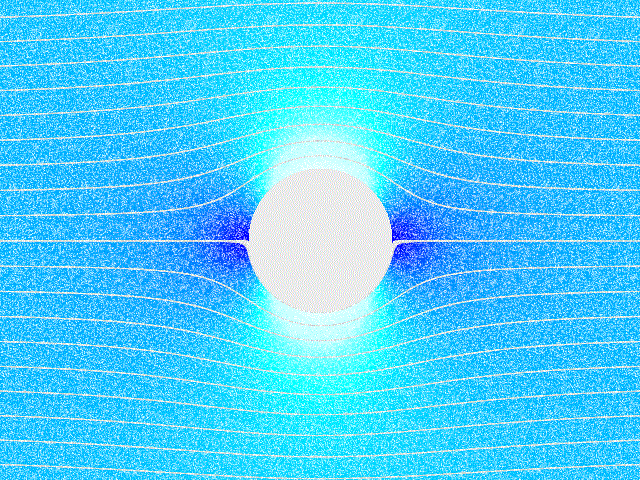
\includegraphics[width=.5\linewidth]{Inviscid_flow_around_a_cylinder-0.png}}

\end{exercise}


\end{document}
